\documentclass[../thesis.tex]{subfiles}

\begin{document}

Μέσα στις απαιτήσεις της εφαρμογής μας συμπεριλαμβάνεται και η αποθήκευση των δεδομένων των χρηστών online.
Για την αποθήκευση των δεδομένων αυτών στον server η ιδανική λύση είναι η χρήση μίας σχεσιακής βάσης δεδομένων τύπου SQL (στην περίπτωσή μας της MySQL). 

Όπως έχουμε αναφέρει, τα δεδομένα που επιθυμούμε να αποθηκεύσουμε στη βάση αφορούν τους χρήστες και τα οχήματά τους.
Ο κάθε χρήστης έχει έναν αριθμό μητρώου, τα οχήματά του, μία βαθμολογία, και μία εικόνα προφίλ.
Οι πληροφορίες του κάθε οχήματος ενός χρήστη περιλαμβάνουν το μοντέλο, τον αριθμό πινακίδας, τον αριθμό θέσεων, το χρώμα, και μία φωτογραφίας.

Είναι σαφές ότι η βάση μας θα αποτελείται από δύο πίνακες/tables, ένα για τους χρήστες, και ένα για τα οχήματα.
Τα απαραίτητα columns που θα διαθέτει ο κάθε πίνακας είναι προφανή.
Εφόσον το κάθε όχημα ανήκει σε έναν ακριβώς χρήστη, και επειδή ο κάθε χρήστης επιτρέπεται να έχει πολλαπλά οχήματα, έχουμε μία σχέση one-to-many μεταξύ χρηστών και οχημάτων.
Για να υλοποιήσουμε τη σχέση αυτή στη βάση, θα προσθέσουμε στις στήλες του πίνακα οχημάτων τον ΑΜ του αντίστοιχου χρήστη-ιδιοκτήτη ως foreign key.

\begin{figure}
    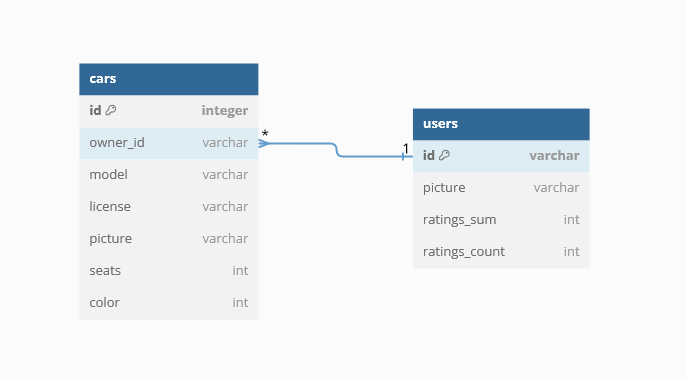
\includegraphics[width=\textwidth]{db_schema.png}
    \centering
    \caption{Σχηματικό διάγραμμα που περιγράφει τη δομή της βάσης δεδομένων που χρησιμοποιούμε. (Δημιουργήθηκε μέσω της ιστοσελίδας \url{dbdiagram.io})}
\end{figure}

Το primary key του πίνακα χρηστών είναι το ΑΜ τους, ενώ το primary key των οχημάτων είναι ένας απλός auto-incrementing ακέραιος.
Εφόσον όλες οι εικόνες είναι αποθηκευμένες ως αρχεία στο δίσκο, η πληροφορία που περιέχεται στη βάση είναι το όνομα/UUID του αρχείου που αντιστοιχεί στην κάθε εικόνα.
Το χρώμα του κάθε οχήματος αναπαριστάται ως ένας 32-bit unsigned integer που αντιστοιχεί στα τέσσερα 8-bit κανάλια ARGB\footnote{Ο λόγος που χρησιμοποιούμε ακέραιο τύπο για το χρώμα αντί για ένα string που αναπαριστά το hex color code είναι το γεγονός ότι το Flutter ορίζει χρώματα μόνο βάσει της ακέραιας 32-bit αναπαράστασής τους, επομένως έτσι αποφεύγουμε τις περιττές μετατροπές τιμών. Εξ άλλου, η αναπαράσταση με ακέραιο στη βάση είναι ελαφρώς πιο αποδοτική από την χρήση string, ωστόσο η διαφορά αυτή δεν είναι τόσο σημαντική.}.
Η βαθμολογία του χρήστη αποθηκεύεται σε δύο μερή, το πλήθος και το άθροισμα των αξιολογήσεων, ώστε να μπορούμε να εξάγουμε και να ενημερώνουμε κατάλληλα τον μέσο όρο.

\bigskip

Η μορφή της βάσης ως έχει είναι αρκετά απλή καθώς δεν υπάρχει η ανάγκη διαχείρησης πιο πολύπλοκων δεδομένων.
Ωστόσο εύκολα μπορεί να επεκταθεί αν οι απαιτήσεις της εφαρμογής γίνουν πιο σύνθετες.
Για παράδειγμα, αν επιθυμούσαμε να καταγράφουμε κάθε διαδρομή στη βάση, θα προσθέταμε έναν επιπλέον πίνακα διαδρομών στον οποίο θα βρίσκονται όλα τα σχετικά δεδομένα της διαδρομής που μας ενδιαφέρουν.
Εκτός από το ID, για την κάθε διαδρομή θα ορίζαμε τον οδηγό και τους επιβάτες οι οποίοι συμμετείχαν σε αυτή, καθώς και το όχημα του οδηγού.
Το ID του οδηγού και του οχήματος εύκολα προστίθονται ως στήλες του πίνακα διαδρομών καθώς και στις δύο περιπτώσεις έχουμε μία σχέση one-to-many.

Οι επιβάτες μίας διαδρομής ωστόσο ορίζουν μία σχέση many-to-many, καθώς πολλοί επιβάτες μπορούν να συμμετέχουν σε μία διαδρομή, και κάθε επιβάτης μπορεί να συμμετάσχει σε πολλές διαδρομές σε διαφορετικές χρονικές στιγμές.
Για αυτό το λόγο απαιτείται η χρήση ενός επιπλέον συνδετικού πίνακα (associative table) ο οποίος θα αναπαριστά τη many-to-many relationship, με ένα foreign key για το ID της διαδρομής και ένα foreign key για τον επιβάτη.

Τέλος, θα μπορούσαμε να εξάγουμε τις αξιολογήσεις των χρηστών σε έναν ξεχωριστό πίνακα, προκειμένου να ενσωματώσουμε όλες τις πληροφορίες της κάθε αξιολόγησης.
Στον πίνακα αυτόν κάθε αξιολόγηση θα ορίζεται από τον συνδυασμό του ID της διαδρομής στην οποία συνέβει, και τα ID του αξιολογητή και αξιολογούμενου.
Εκτός από τον αριθμό αστεριών, μπορούμε επίσης να προσθέσουμε μία στήλη για επιπλέον σχόλια του αξιολογητή.

\begin{figure}
    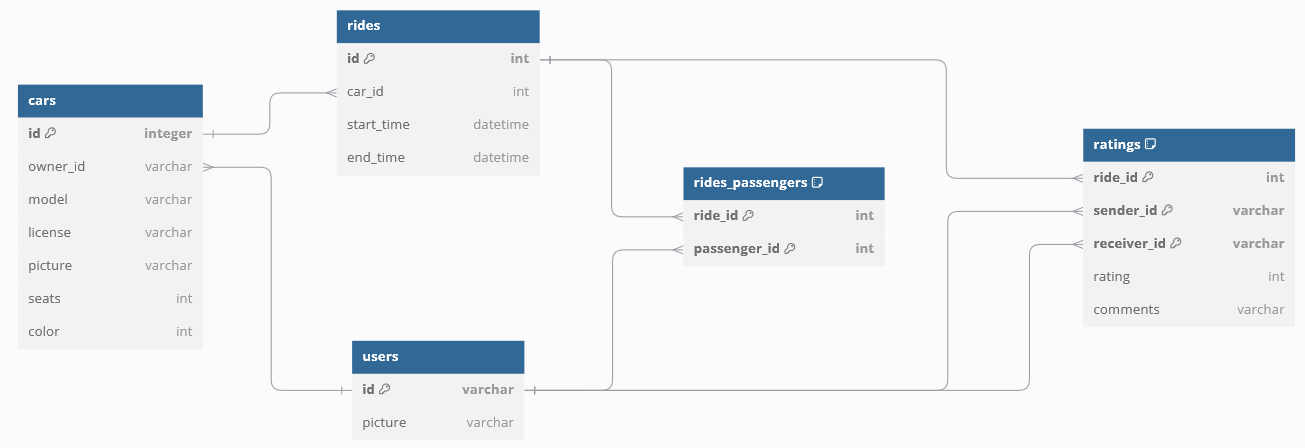
\includegraphics[width=\textwidth]{db_schema_complex.png}
    \centering
    \caption{Σχηματικό διάγραμμα που περιγράφει μία εναλλακτική, πιο σύνθετη δομή για τη βάση δεδομένων που μπορούμε να χρησιμοποιήσουμε αν η εφαρμογή επεκταθεί στο μέλλον}
\end{figure}

\end{document}